\documentclass[aspectratio=169,11pt,xcolor=table]{beamer}
\usetheme{Berlin}
\setbeamertemplate{headline}{}
\usepackage[no-math]{fontspec}
\usepackage{amsmath,amssymb,icomma,bm,booktabs,tabularx,graphicx}
\definecolor{navy}{rgb}{0.2,0.2,0.7}
\definecolor{ods}{HTML}{00689D}
\definecolor{destaque}{HTML}{C8343B}
\definecolor{verde}{HTML}{2E7D4F}
\definecolor{fundo}{HTML}{EAF1F7}
\setbeamercolor{alerted text}{fg=destaque}
\setbeamerfont{institute}{size=\footnotesize}
\setbeamerfont{date}{size=\footnotesize}
\setbeamertemplate{navigation symbols}{}
\setbeamertemplate{footline}{\hspace{1em}\scriptsize\color{black!55}GED-16 · Homicídios nos municípios\hfill\insertframenumber\hspace{1em}\vspace{0.6em}}
\graphicspath{{figuras/}{../../entrega/resultados/eda/}{../../entrega/resultados/modelagem/}}
\newcommand{\fig}[1]{\includegraphics[width=\linewidth,height=0.62\textheight,keepaspectratio]{#1}}
\newcommand{\fonte}[1]{\par\vspace{0.2em}{\tiny\color{black!65}Fonte: #1\par}}
\newcommand{\nLambdaFinal}{0,17}
\newcommand{\nLambdaFinalInf}{0,12}
\newcommand{\nLambdaFinalSup}{0,23}
\newcommand{\nPMigrFinal}{0,143}
\newcommand{\nPMigrAntiga}{0,043}
\newcommand{\nPMigrCorrigida}{0,147}
\newcommand{\nMunBR}{5.570}
\newcommand{\nHomBR}{138.316}
\newcommand{\nTaxaBR}{22,7}
\newcommand{\nPopMin}{30}
\newcommand{\nMunEsc}{1.133}
\newcommand{\nPctPopEsc}{77}
\newcommand{\nPercCorte}{80}
\newcommand{\nPctMaiores}{20}
\newcommand{\nCasosEspCorte}{20}
\newcommand{\nFDens}{0,08}
\newcommand{\nPDens}{0,78}
\newcommand{\nForaNome}{Campos do Jordão-SP}
\newcommand{\nForaHom}{1}
\newcommand{\nForaIndet}{36}
\newcommand{\nGiniZero}{931}
\newcommand{\nGiniZeroPct}{29}
\newcommand{\nGiniEfMediana}{$+$16}
\newcommand{\nGiniEfNoventa}{$+$34}
\newcommand{\nCorDesocup}{$+$0,30}
\newcommand{\nCorDesocupRenda}{$-$0,55}
\newcommand{\nRdoisPct}{56}
\newcommand{\nSWpEstado}{$<$0,001}
\newcommand{\nFInter}{64,6}
\newcommand{\nRdoisAsemInter}{0,53}
\newcommand{\nPMigr}{0,14}
\newcommand{\nZerosBR}{655}
\newcommand{\nTaxaMedia}{24,7}
\newcommand{\nTaxaMediana}{20,4}
\newcommand{\nTaxaQuartilUm}{11,2}
\newcommand{\nTaxaQuartilTres}{35,0}
\newcommand{\nAssimTaxa}{1,25}
\newcommand{\nHomAno}{46.105}
\newcommand{\nTaxaMundo}{5,8}
\newcommand{\nRazaoMundo}{3,9}
\newcommand{\nTaxaNbr}{36,4}
\newcommand{\nTaxaNEbr}{36,9}
\newcommand{\nTaxaCObr}{22,2}
\newcommand{\nTaxaSEbr}{13,0}
\newcommand{\nTaxaSbr}{16,7}
\newcommand{\nCorMax}{0,49}
\newcommand{\nCorMaxVar}{Distorção EM}
\newcommand{\nCorTrio}{0,91}
\newcommand{\nRendaDecilPico}{873}
\newcommand{\nDecilPico}{3}
\newcommand{\nPicoPct}{20}
\newcommand{\nRendaMediana}{1.383}
\newcommand{\nPorteHomMenor}{1}
\newcommand{\nPorteOscMenor}{66}
\newcommand{\nPorteOscCorte}{20}
\newcommand{\nLambda}{0,21}
\newcommand{\nLambdaInf}{0,15}
\newcommand{\nLambdaSup}{0,26}
\newcommand{\nSWy}{0,93}
\newcommand{\nSWln}{0,99}
\newcommand{\nVIFrenda}{16}
\newcommand{\nRdoisA}{0,56}
\newcommand{\nFblocoEd}{68,0}
\newcommand{\nRdoisAsemEd}{0,35}
\newcommand{\nRdoisAcomEd}{0,43}
\newcommand{\nFglobal}{111}
\newcommand{\nGlUm}{13}
\newcommand{\nGlDois}{1.119}
\newcommand{\nPico}{815}
\newcommand{\nBP}{46}
\newcommand{\nSW}{0,998}
\newcommand{\nNout}{0}
\newcommand{\nSWp}{0,165}
\newcommand{\nBPgl}{13}
\newcommand{\nBPp}{$<$0,001}
\newcommand{\nRdoisE}{0,56}
\newcommand{\nSigma}{0,524}
\newcommand{\nFglobalP}{$<$0,001}
\newcommand{\nVIFrendaFinal}{7,6}
\newcommand{\nVIFdemaisMax}{3,1}
\newcommand{\nVIFrendaCru}{1.289}
\newcommand{\nGiniCorUF}{0,995}
\newcommand{\nGiniErroUF}{0,003}
\newcommand{\nNumReg}{4}
\newcommand{\nNumX}{5}
\newcommand{\nNumPar}{14}
\newcommand{\nCorQuadSem}{0,9994}
\newcommand{\nCorQuadCen}{$-$0,20}
\newcommand{\nBetaDois}{$-$0,998}
\newcommand{\nBetaDoisP}{$<$0,001}
\newcommand{\nOutNomes}{nenhum}
\newcommand{\nGiniEfDez}{$-$10}
\newcommand{\nGiniEfVinteCinco}{$-$2}
\newcommand{\nRendaDez}{699}
\newcommand{\nRendaNoventa}{2.043}
\newcommand{\nEscolaEfeito}{$-$8,6}
\newcommand{\nDistorcaoEfeito}{$+$15,6}
\newcommand{\nUrbanaEfeito}{$+$11,8}
\newcommand{\nFRenda}{74,5}
\newcommand{\nGlRenda}{3}
\newcommand{\nPRenda}{$<$0,001}
\newcommand{\nRdoisAsemRenda}{0,47}
\newcommand{\nVIFmaxSemRenda}{1,8}
\newcommand{\nNumParEstado}{36}
\newcommand{\nRdoisAestado}{0,64}
\newcommand{\nVIFmaxEstado}{10,6}
\newcommand{\nFEstado}{12,1}
\newcommand{\nGlEstado}{22}
\newcommand{\nPEstado}{$<$0,001}
\newcommand{\nNumUFpoucos}{5}
\newcommand{\nNaoSig}{migração recente}

\title{Fatores associados aos homicídios nos municípios brasileiros}
\subtitle{Regressão linear múltipla · ODS 16}
\author{\footnotesize Douglas Bergamim Fernandes \and Fabio Eiiti Kobayashi Urio \and Kauan Alves Aragão \and Luiz Felipe de Brito Ramos \and Willian Nelton Teleken}
\institute{Instituto Tecnológico de Aeronáutica · GED-16 Análise de Regressão}
\date{Apresentação final · 18 de novembro de 2026}
\begin{document}
\maketitle

\section{Contexto e pergunta}
\begin{frame}{Contexto e questão de pesquisa}
\begin{itemize}
\setlength{\itemsep}{0.5em}
\item Brasil, 2021--2023: \textbf{\nHomAno{} mortes por ano} na medida do estudo
\item A violência letal se distribui de forma desigual entre as regiões
\item ODS 16: reduzir a violência e as mortes relacionadas
\end{itemize}
\begin{block}{Pergunta}
Quais características socioeconômicas, demográficas e geográficas estão associadas à taxa de homicídios nos municípios brasileiros?
\end{block}
{\small Hipóteses: desigualdade (H1), exclusão escolar (H2) e migração recente (H3) associadas a taxas maiores.}
\fonte{SIM/DATASUS; IBGE. Hipóteses: Fajnzylber et al. (2002), Lochner e Moretti (2004), Sampson e Groves (1989).}
\end{frame}

\section{Dados}
\begin{frame}{Fontes e medida de violência}
\begin{tabularx}{\linewidth}{@{}>{\raggedright\arraybackslash}p{0.24\linewidth}X@{}}
\toprule
\textbf{Fonte} & \textbf{O que utilizamos}\\
\midrule
SIM/DATASUS & Óbitos por residência, média anual de 2021--2023\\[0.4em]
IBGE, Censo 2022 & População, renda, desigualdade, trabalho, urbanização, frequência escolar e migração\\[0.4em]
INEP, 2022 & Distorção idade-série no ensino médio\\
\bottomrule
\end{tabularx}
\vspace{0.5em}
\[
\text{Taxa anual} = \frac{\text{óbitos em 2021--2023}}{3\,\times\,\text{população de 2022}}\,\times\,100\,000
\]
{\small Agressões (X85--Y09) + intervenções legais/operações de guerra (Y35--Y36).}
\fonte{SIM/DATASUS; IBGE; INEP. Medida relacionada ao ODS 16; a definição difere do indicador oficial 16.1.1.}
\end{frame}

\begin{frame}{Recorte e variáveis do modelo}
\begin{columns}[T]
\column{0.48\textwidth}
\textbf{\color{ods}Onde o modelo se aplica}
\begin{itemize}
\item Municípios com \nPopMin{} mil habitantes ou mais
\item \textbf{\nMunEsc{} municípios}: \nPctPopEsc\% da população brasileira
\item Corte próximo do percentil \nPercCorte{} da população municipal
\item \nForaNome{} excluído por indício de sub-registro
\end{itemize}
\column{0.48\textwidth}
\textbf{\color{ods}Cinco grupos de explicativas}
\begin{itemize}
\item Renda, Gini e desocupação
\item Urbanização
\item Frequência e atraso escolar
\item Migração recente
\item Região, com referência no Sudeste
\end{itemize}
\end{columns}
\vspace{0.5em}
{\small Gini: aproximação pelas classes de renda. Migração: moradores há menos de dez anos no município.}
\fonte{Elaboração própria. Cidades menores têm taxas mais instáveis; o recorte não elimina todo problema de registro.}
\end{frame}

\section{Padrões nos dados}
\begin{frame}{A distribuição da taxa difere entre regiões}
\begin{columns}[c]
\column{0.64\textwidth}
\fig{e3_box_regiao.png}
\column{0.33\textwidth}
\begin{itemize}
\item Norte e Nordeste têm medianas maiores no recorte
\item Há diferenças entre municípios da mesma região
\item Região sozinha não explica essa variação
\end{itemize}
\end{columns}
\fonte{SIM/DATASUS; IBGE. Eixo em ln(taxa). Linha central: mediana; caixa: metade central; ponto vermelho: média de ln(taxa).}
\end{frame}

\begin{frame}{A relação bruta com a renda não é uma reta}
\begin{columns}[c]
\column{0.64\textwidth}
\fig{e7_box_renda.png}
\column{0.33\textwidth}
\begin{itemize}
\item A mediana é maior em uma faixa intermediária de renda
\item O padrão sugere uma relação curva
\item Ainda não controlamos as outras características
\end{itemize}
\end{columns}
\fonte{SIM/DATASUS; IBGE. Eixo em ln(taxa). Décimos de renda per capita; pontos vermelhos: médias de ln(taxa).}
\end{frame}

\section{Método e diagnóstico}
\begin{frame}{Modelo ajustado e finalidade dos métodos}
\begin{itemize}
\setlength{\itemsep}{0.65em}
\item \textbf{Regressão linear múltipla para ln(taxa):} comparar municípios mantendo outras características constantes
\item \textbf{Renda ao quadrado:} representar a relação curva; \textbf{Gini $\times$ renda:} permitir que a associação da desigualdade mude com a renda
\item \textbf{Testes $F$:} avaliar a contribuição do modelo e dos termos acrescentados
\item \textbf{Resíduos e gráficos:} avaliar a forma dos erros; VIF entra depois como alerta para a leitura dos coeficientes
\end{itemize}
\vspace{0.4em}
{\small Ajuste final: $R^2$ ajustado = \nRdoisA, \textbf{na escala de ln(taxa)}.}
\fonte{Elaboração própria. Apostila GED-16, caps. 4, 6 e 7. Box-Cox e comparação de modelos nos apêndices.}
\end{frame}

\begin{frame}{Diagnóstico: o tamanho dos erros ainda varia}
\begin{columns}[c]
\column{0.49\textwidth}
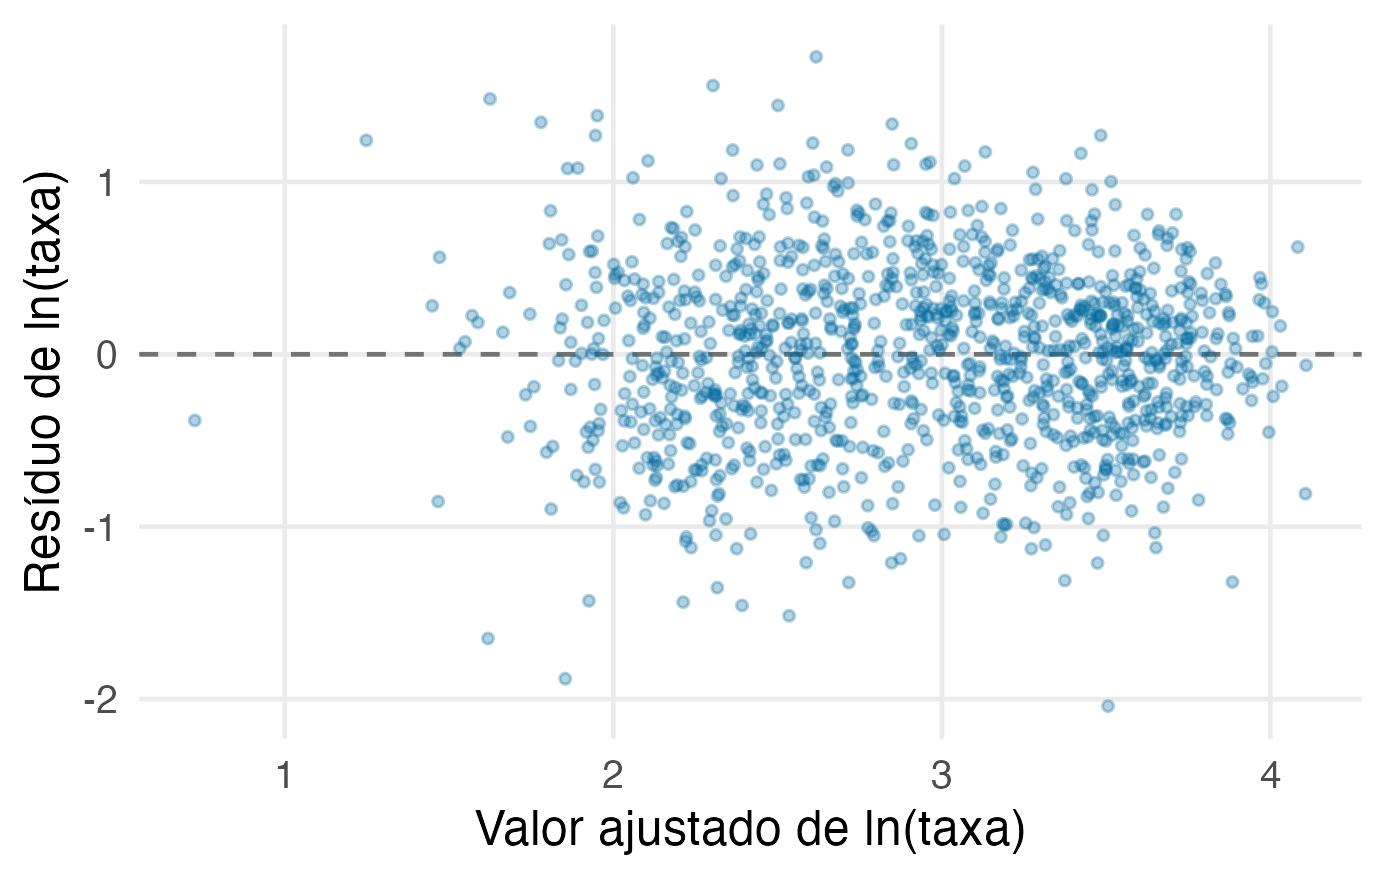
\includegraphics[width=\linewidth]{residuos_ajustado.png}
\column{0.49\textwidth}
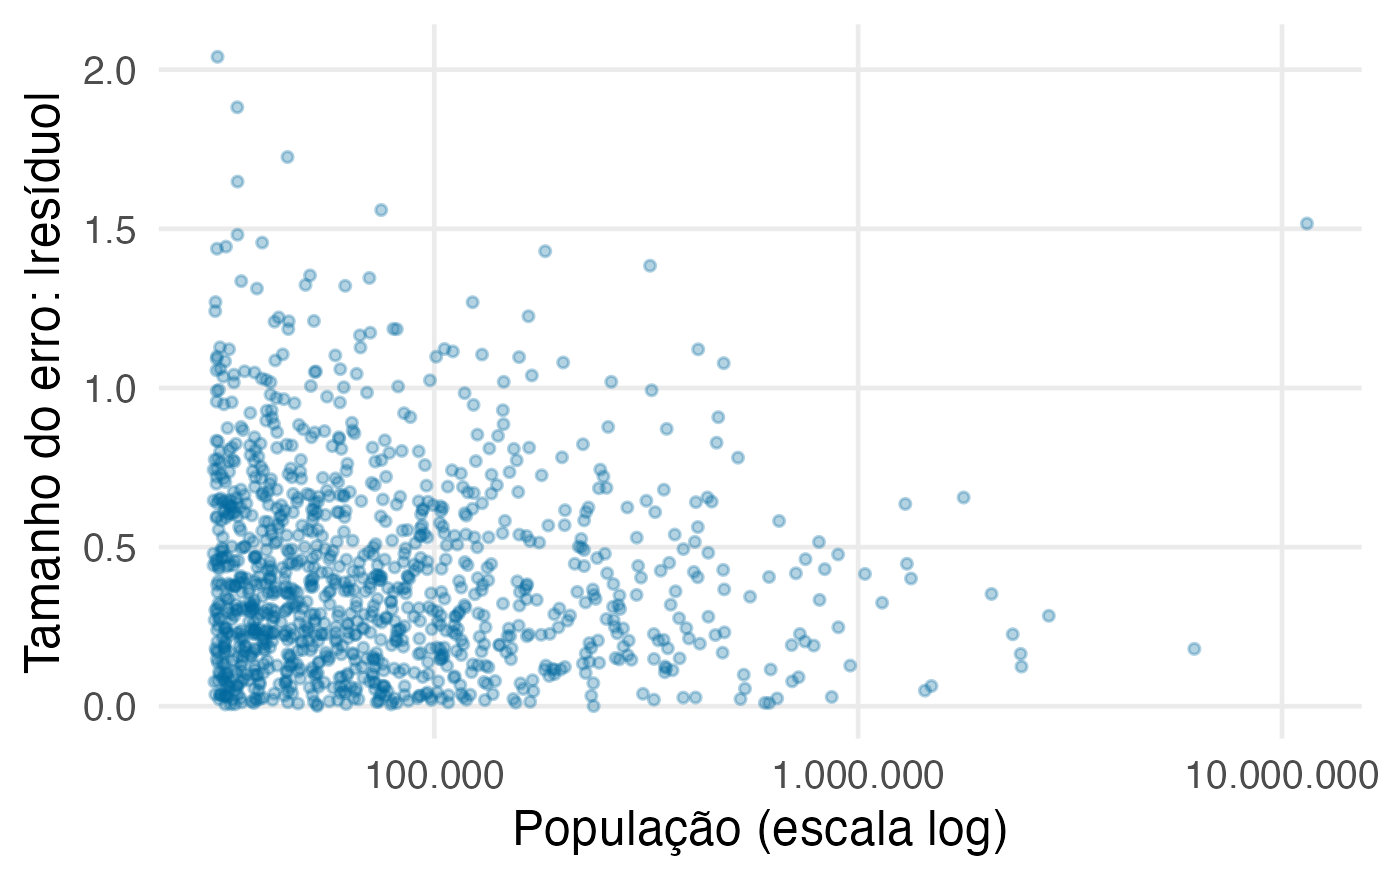
\includegraphics[width=\linewidth]{residuos_populacao.png}
\end{columns}
\vspace{0.2em}
{\small \textbf{Leitura:} procurar uma faixa sem curva e com largura constante. A dispersão diminui com a população.}
\vspace{0.3em}
{\small \alert{Breusch-Pagan rejeita variância constante.} Intervalos e testes clássicos exigem cautela.}
\fonte{Modelo final. Linha tracejada: erro zero. Breusch-Pagan: $p$ \nBPp. Cada ponto representa um município.}
\end{frame}

\begin{frame}{Diagnóstico: os resíduos se aproximam da normal}
\begin{columns}[c]
\column{0.49\textwidth}
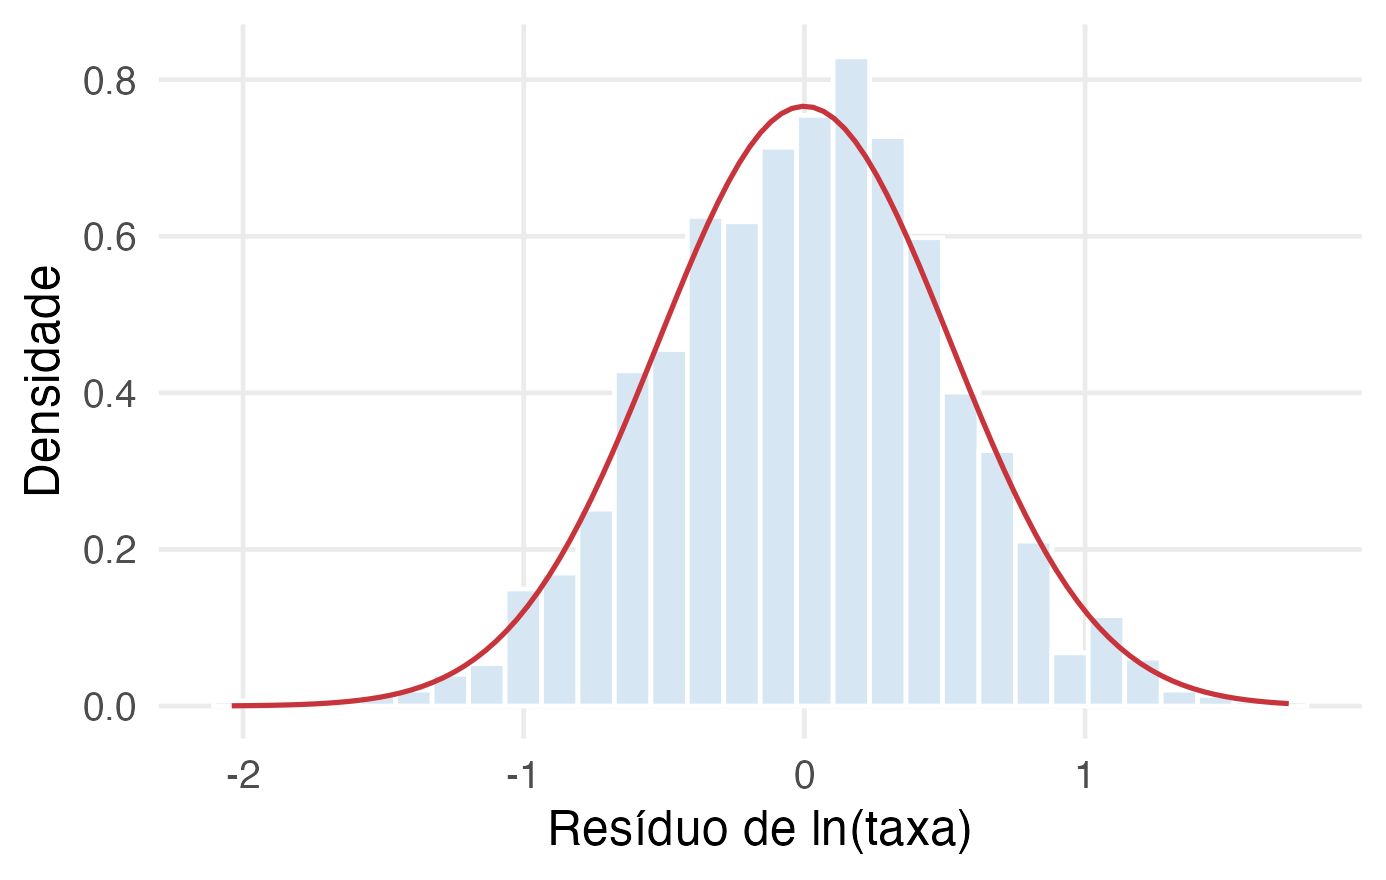
\includegraphics[width=\linewidth]{histograma_residuos.png}
\column{0.49\textwidth}
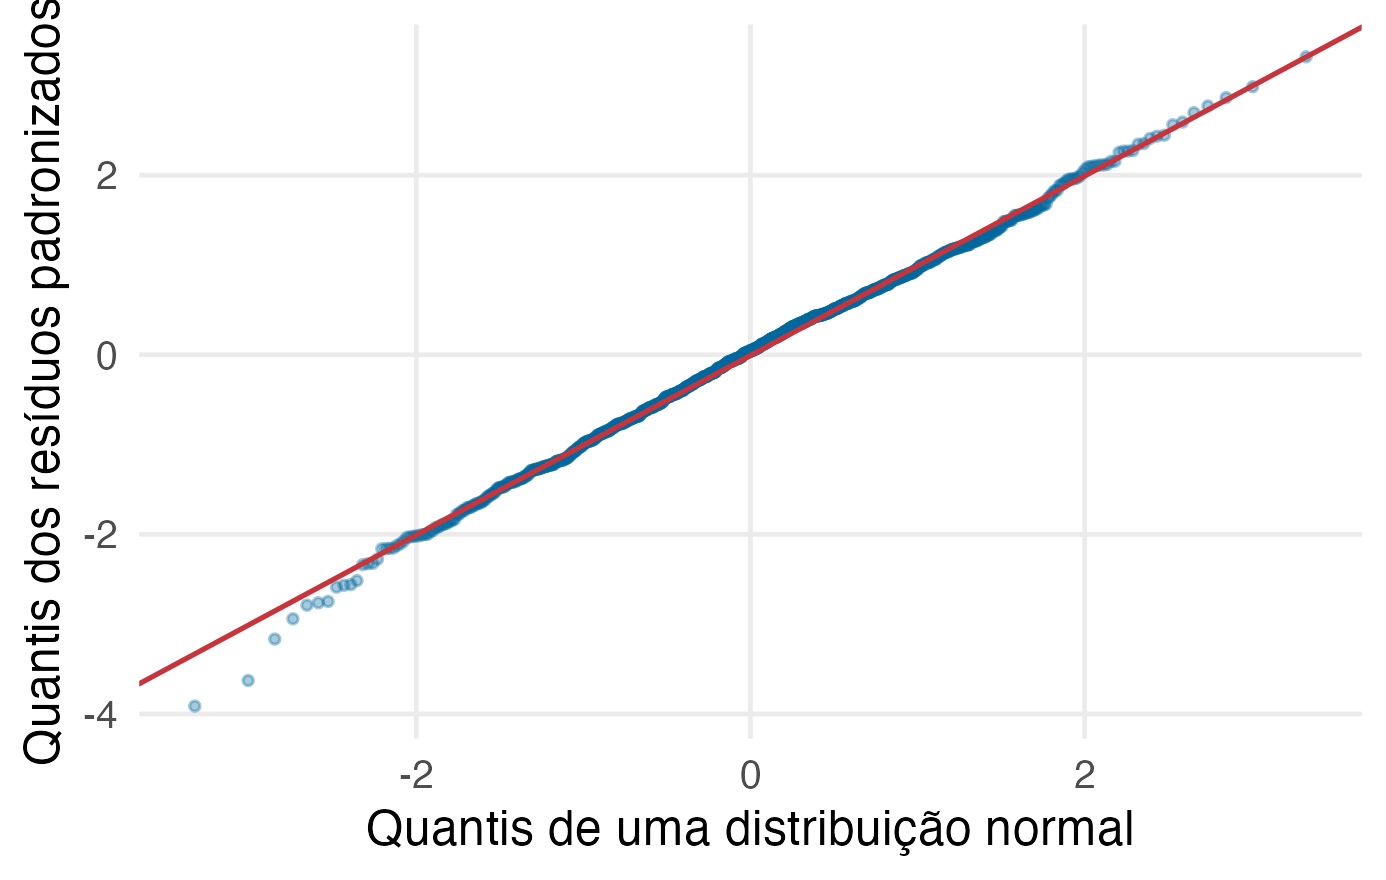
\includegraphics[width=\linewidth]{qq_final.png}
\end{columns}
\vspace{0.2em}
{\small \textbf{Leitura:} o histograma acompanha a curva; no gráfico de quantis, os pontos ficam próximos da reta.}
\vspace{0.3em}
{\small Shapiro-Wilk não rejeita normalidade ($p$ = \nSWp). \textbf{Isso não resolve a variância não constante.}}
\fonte{Modelo final. Quantis comparam a distribuição dos resíduos com uma normal. Normalidade não é comprovada pelo teste.}
\end{frame}

\section{Resultados e discussão}
\begin{frame}{Escola e urbanização têm associações claras no ajuste}
\begin{columns}[c]
\column{0.68\textwidth}
\fig{efeitos.png}
\column{0.29\textwidth}
\begin{itemize}\small
\item Mais frequência escolar: taxa menor
\item Mais atraso escolar: taxa maior
\item Migração: intervalo cruza zero
\end{itemize}
\end{columns}
\fonte{Elaboração própria. p.p. = pontos percentuais. Pontos: estimativas; barras: IC 95\% clássico, sem correção de variância. Associação, não causa.}
\end{frame}

\begin{frame}{A associação da desigualdade muda com a renda}
\begin{columns}[c]
\column{0.65\textwidth}
\fig{gini_renda.png}
\column{0.32\textwidth}
\begin{itemize}\small
\item Efeito estimado de +0,05 no Gini
\item Na renda mediana: \textbf{\nGiniEfMediana\%}
\item No percentil 90 da renda: \textbf{\nGiniEfNoventa\%}
\item Na baixa renda, o sinal varia; não há um efeito positivo geral
\end{itemize}
\end{columns}
\fonte{Elaboração própria. Faixa: IC 95\% clássico, sem correção de variância. Pontos vermelhos: percentis 10, 50 e 90 da renda.}
\end{frame}

\begin{frame}{Renda e região permanecem associadas à taxa}
\begin{columns}[c]
\column{0.65\textwidth}
\fig{renda_regiao.png}
\column{0.32\textwidth}
\begin{itemize}\small
\item Curva da renda no Gini médio
\item Pico estimado perto de R\$ \nPico
\item Nordeste acima do Sudeste com outras características iguais
\item O gráfico mostra a taxa típica retransformada
\end{itemize}
\end{columns}
\fonte{Elaboração própria. Curvas restritas à renda observada em cada região. Faixas: IC 95\% clássico. Não representam média aritmética da taxa.}
\end{frame}

\begin{frame}{Limitações que restringem as conclusões}
\begin{itemize}
\setlength{\itemsep}{0.5em}
\item \textbf{Variância não constante:} tratar os intervalos e testes como evidência exploratória
\item \textbf{Medição:} Gini aproximado e possível sub-registro dos óbitos; cidades pequenas ficam fora do recorte
\item \textbf{Desocupação:} associação negativa frágil; o sinal não demonstra sua causa
\item \textbf{Vizinhança:} municípios próximos podem compartilhar fatores; independência espacial não foi verificada
\item \textbf{Estudo observacional:} associação municipal não demonstra causa nem descreve indivíduos
\end{itemize}
\fonte{Diagnóstico do modelo e validação dos dados. VIF máximo \nVIFrendaFinal; esse número não substitui a análise dos resíduos.}
\end{frame}

\begin{frame}{Resposta à pergunta e próximos passos}
\begin{itemize}
\setlength{\itemsep}{0.5em}
\item \textbf{Desigualdade:} associação positiva nas rendas média e alta; depende da renda do município
\item \textbf{Escola:} frequência e atraso escolar apresentam associações nas direções esperadas
\item \textbf{Migração:} não encontramos evidência clara no modelo ajustado
\item \textbf{Literatura:} escola e desigualdade têm respaldo; diferenças regionais também aparecem em estudos municipais
\item \textbf{Próximos passos:} tratar a variância dos erros e ampliar informações sobre políticas estaduais e violência organizada
\end{itemize}
\fonte{Fajnzylber et al. (2002); Lochner e Moretti (2004); Wanzinack et al. (2022); Barros et al. (2020). Resultados são associações.}
\end{frame}

\appendix
\begin{frame}{Apêndice A · Coeficientes do modelo final}
\scriptsize
\renewcommand{\arraystretch}{1.02}
\begin{tabular*}{\textwidth}{@{\extracolsep{\fill}}lrrrlrrr@{}}
\toprule
\textbf{Termo} & \textbf{$b$} & \textbf{EP} & \textbf{$p$} & \textbf{Termo} & \textbf{$b$} & \textbf{EP} & \textbf{$p$}\\
\midrule
Intercepto & 3,021 & 0,337 & $<$0,001 & Freq. escolar 15--17 & $-$0,018 & 0,004 & $<$0,001\\
ln(renda) centr. & $-$0,861 & 0,101 & $<$0,001 & Distorção EM & 0,014 & 0,002 & $<$0,001\\
(ln(renda) centr.)² & $-$0,998 & 0,092 & $<$0,001 & Migração recente & 0,004 & 0,003 & 0,143\\
Desigualdade (Gini, centr.) & 2,209 & 0,481 & $<$0,001 & Norte & 0,580 & 0,082 & $<$0,001\\
Gini $\times$ ln(renda) & 7,398 & 0,921 & $<$0,001 & Nordeste & 0,731 & 0,061 & $<$0,001\\
Desocupação & $-$0,018 & 0,008 & 0,022 & Centro-Oeste & 0,603 & 0,070 & $<$0,001\\
\% urbana & 0,011 & 0,002 & $<$0,001 & Sul & 0,515 & 0,055 & $<$0,001\\
\bottomrule
\end{tabular*}

\fonte{Elaboração própria. Resposta ln(taxa); erros-padrão e testes clássicos, sem correção de variância.}
\end{frame}

\begin{frame}{Apêndice B · Testes e contribuição dos termos}
\begin{columns}[T]
\column{0.54\textwidth}
\scriptsize
\renewcommand{\arraystretch}{1.25}
\setlength{\tabcolsep}{2pt}
\begin{tabular}{@{}lrrrr@{}}
\toprule
\textbf{Bloco} & \textbf{gl} & \textbf{$F$ parcial} & \textbf{$p$} & \textbf{$R^2_a$}\\
\midrule
A: renda e desigualdade & --- & --- & --- & 0,28\\
B: + demografia & 4 & 69,8 & $<$0,001 & 0,34\\
C: + fronteira e registro & 2 & 90,4 & $<$0,001 & 0,39\\
D: + educação e migração & 4 & 41,6 & $<$0,001 & 0,43\\
\rowcolor{fundo}\textbf{E: + estado (UF)} & \textbf{26} & \textbf{24,0} & \textbf{$<$0,001} & \textbf{0,58}\\
\bottomrule
\end{tabular}

\column{0.43\textwidth}
\begin{itemize}\small
\item $F$ global: \nFglobal, $p$ \nFglobalP
\item Shapiro-Wilk: $p$ = \nSWp
\item Breusch-Pagan: $p$ \nBPp
\item Nenhum resíduo semi-studentizado além de $\pm4$
\item VIF máximo: \nVIFrendaFinal
\end{itemize}
\end{columns}
\vspace{0.5em}
{\small Os gráficos dos slides 8 e 9 explicam os diagnósticos. Não foi realizado teste de independência espacial.}
\fonte{Elaboração própria. Testes clássicos; interpretar com cautela pela variância não constante.}
\end{frame}

\begin{frame}{Apêndice C · Transformação da resposta (Box-Cox)}
\begin{columns}[c]
\column{0.62\textwidth}
\fig{m1_boxcox.png}
\column{0.35\textwidth}
\begin{itemize}\small
\item Melhor potência: \nLambda
\item IC 95\%: [\nLambdaInf; \nLambdaSup]
\item O log corresponde a zero, fora do intervalo
\item Escolha do log: leitura percentual e melhora visual dos resíduos
\end{itemize}
\end{columns}
\fonte{Elaboração própria. Box-Cox no modelo auxiliar anterior aos termos quadrático e de interação. Não selecionou log como potência ótima.}
\end{frame}

\begin{frame}{Apêndice D · Modelo com e sem a renda}
\begin{columns}[c]
\column{0.56\textwidth}
\scriptsize
\renewcommand{\arraystretch}{1.15}
\setlength{\tabcolsep}{3pt}
\begin{tabular}{@{}lrrrr@{}}
\toprule
 & \multicolumn{2}{c}{\textbf{Com renda}} & \multicolumn{2}{c}{\textbf{Sem renda}}\\
\textbf{Termo} & \textbf{$b$} & \textbf{$p$} & \textbf{$b$} & \textbf{$p$}\\
\midrule
Desigualdade (Gini) & 3,006 & $<$0,001 & 0,858 & 0,045\\
Desocupação & $-$0,005 & 0,473 & 0,010 & 0,119\\
\% urbana & 0,010 & $<$0,001 & 0,011 & $<$0,001\\
\textbf{ln densidade (padr.)} & \textbf{0,054} & \textbf{0,021} & \textbf{$-$0,033} & \textbf{0,153}\\
\% homens 15--29 & $-$0,033 & 0,067 & $-$0,018 & 0,296\\
Fronteira & $-$0,038 & 0,552 & $-$0,042 & 0,536\\
\% indeterminada & $-$0,008 & $<$0,001 & $-$0,005 & 0,031\\
Freq. escolar 15--17 & $-$0,016 & $<$0,001 & $-$0,017 & $<$0,001\\
Abandono EM & $-$0,002 & 0,538 & $-$0,005 & 0,245\\
Distorção EM & 0,010 & $<$0,001 & 0,014 & $<$0,001\\
\textbf{Migração recente} & \textbf{0,009} & \textbf{0,001} & \textbf{0,004} & \textbf{0,150}\\
\bottomrule
\end{tabular}

\column{0.41\textwidth}
\begin{itemize}\small
\item Renda mantida: contribuição conjunta de renda, renda² e Gini $\times$ renda
\item $F$ parcial: \nFRenda; $p$ \nPRenda
\item $R^2_a$: \nRdoisA{} com renda; \nRdoisAsemRenda{} sem renda
\item A comparação não isola apenas a renda linear
\end{itemize}
\end{columns}
\fonte{Elaboração própria. Indicadoras de região omitidas; ao retirar renda, sai a interação. Inferência clássica.}
\end{frame}

\begin{frame}{Apêndice E · Região escolhida; estado como comparação}
\begin{columns}[c]
\column{0.55\textwidth}
\scriptsize
\renewcommand{\arraystretch}{1.1}
\setlength{\tabcolsep}{3pt}
\begin{tabular}{@{}lrrrr@{}}
\toprule
 & \multicolumn{2}{c}{\textbf{Com região}} & \multicolumn{2}{c}{\textbf{Com estado}}\\
\textbf{Termo} & \textbf{$b$} & \textbf{$p$} & \textbf{$b$} & \textbf{$p$}\\
\midrule
ln(renda) centr. & $-$0,861 & $<$0,001 & $-$0,549 & $<$0,001\\
(ln(renda) centr.)² & $-$0,998 & $<$0,001 & $-$0,701 & $<$0,001\\
\textbf{Desigualdade (Gini)} & \textbf{2,209} & \textbf{$<$0,001} & \textbf{0,729} & \textbf{0,119}\\
Desocupação & $-$0,018 & 0,022 & $-$0,015 & 0,047\\
\% urbana & 0,011 & $<$0,001 & 0,012 & $<$0,001\\
Freq. escolar 15--17 & $-$0,018 & $<$0,001 & $-$0,014 & $<$0,001\\
Distorção EM & 0,014 & $<$0,001 & 0,010 & $<$0,001\\
Migração recente & 0,004 & 0,143 & 0,005 & 0,064\\
Gini $\times$ ln(renda) & 7,398 & $<$0,001 & 5,227 & $<$0,001\\
\bottomrule
\end{tabular}

\column{0.42\textwidth}
\begin{itemize}\small
\item Região: \nNumPar{} parâmetros; $R^2_a$ = \nRdoisA
\item Estado: \nNumParEstado{} parâmetros; $R^2_a$ = \nRdoisAestado
\item O maior ajuste não decide sozinho a escolha
\item Região responde ao objetivo da apresentação com menos parâmetros
\item Referência: Sudeste no modelo final; SP no comparativo
\end{itemize}
\end{columns}
\fonte{Elaboração própria. Decisão do grupo em 17/11/2026. Comparação preservada para perguntas.}
\end{frame}

\begin{frame}{Apêndice F · Variáveis testadas e retiradas}
\footnotesize
\renewcommand{\arraystretch}{1.2}
\begin{tabular}{@{}p{0.36\textwidth}rrp{0.40\textwidth}@{}}
\toprule
\textbf{Variável} & \textbf{$F$} & \textbf{$p$} & \textbf{Motivo da retirada}\\
\midrule
Densidade (ln, padronizada) & 0,08 & 0,782 & Sem evidência adicional\\
Faixa de fronteira & 1,05 & 0,307 & Sem evidência adicional\\
Abandono no ensino médio & 0,19 & 0,667 & Sem evidência adicional\\
\% homens 15--29 & 2,17 & 0,141 & Sem evidência adicional\\
Amazônia Legal & 7,59 & 0,006 & O efeito vem só do Mato Grosso\\
\% intenção indeterminada (sem os homicídios no total) & 0,00 & 0,996 & A medida original tinha os homicídios no divisor; corrigida, sem evidência adicional\\
\bottomrule
\end{tabular}

\fonte{Elaboração própria. $F$ parcial de cada variável somada ao modelo final. Inferência clássica.}
\vspace{0.4em}
{\small \nForaNome: \nForaHom{} homicídio e \nForaIndet{} óbitos de intenção indeterminada em três anos. Exclusão por indício de sub-registro.}
\end{frame}

\begin{frame}{Apêndice G · Métodos fora da apostila}
\scriptsize
\renewcommand{\arraystretch}{1.3}
\begin{tabularx}{\linewidth}{@{}>{\raggedright\arraybackslash}p{0.56\linewidth}X@{}}
\toprule
\textbf{Item} & \textbf{Origem e finalidade}\\
\midrule
Gini municipal calculado pelas classes de renda & Revisão da professora; medir desigualdade\\
Corte próximo do percentil \nPercCorte{} da população & Revisão da professora; definir recorte\\
Padronização de ln(densidade), testada e retirada & Revisão da professora; avaliar extremos\\
VIF generalizado & Grupo; tratar variáveis categóricas\\
$100[\exp(b\Delta)-1]$ & Grupo; ler efeitos percentuais\\
IC da potência Box-Cox & Grupo; explicitar incerteza da transformação\\
Oscilação por porte: $1/\sqrt{\text{casos esperados}}$ & Grupo; apoiar o recorte\\
IC do efeito do Gini por renda & Grupo; interpretar a interação\\
\bottomrule
\end{tabularx}
\fonte{Apostila GED-16 e registro das escolhas do grupo. Nenhum novo modelo foi introduzido nesta revisão.}
\end{frame}

\begin{frame}{Apêndice H · Referências}
\footnotesize
\begin{itemize}
\item FAJNZYLBER, P.; LEDERMAN, D.; LOAYZA, N. Inequality and violent crime. \textit{Journal of Law and Economics}, 45(1), 1--39, 2002.
\item LOCHNER, L.; MORETTI, E. The effect of education on crime. \textit{American Economic Review}, 94(1), 155--189, 2004.
\item SAMPSON, R. J.; GROVES, W. B. Community structure and crime: testing social-disorganization theory. \textit{American Journal of Sociology}, 94(4), 774--802, 1989.
\item WANZINACK, C.; SIGNORELLI, M. C.; REIS, C. Violence and social determinants of health in Brazil. \textit{Cadernos de Saúde Pública}, 38(10), e00282621, 2022.
\item BARROS, P. H. B.; BAGGIO, H. S.; BAGGIO, I. S. The socioeconomic determinants of crime in Brazil. \textit{Revista Brasileira de Segurança Pública}, 14(2), 188--209, 2020.
\end{itemize}
\end{frame}

\begin{frame}{Apêndice I · Métodos e fontes}
\footnotesize
\begin{itemize}
\item FERRARI, D. \textit{Apostila GED-16: Análise de Regressão}. ITA. Caps. 1, 4, 6 e 7.
\item BOX, G. E. P.; COX, D. R. An analysis of transformations. \textit{JRSS, Series B}, 26(2), 211--252, 1964.
\item GASTWIRTH, J. L. The estimation of the Lorenz curve and Gini index. \textit{Review of Economics and Statistics}, 54(3), 306--316, 1972.
\item IBGE. Censo Demográfico 2022, tabelas SIDRA indicadas no dicionário de dados.
\item Ministério da Saúde. SIM/DATASUS, óbitos por residência, 2021--2023.
\item INEP. Indicadores Educacionais 2022: distorção idade-série no ensino médio.
\item ONU/UNODC. Metadados do indicador 16.1.1. A definição oficial não inclui Y35--Y36.
\end{itemize}
\end{frame}
\end{document}
